\documentclass[12pt]{article}
\usepackage{graphicx}
\usepackage{float}
\usepackage[left=2cm,right=2cm]{geometry}
\usepackage[font=scriptsize]{caption}
\graphicspath{{../results/}}

\begin{document}

\textbf{Is Florida getting warmer?}





The observed correlation coefficient between years and temperature of Florida was 0.5331784 (Figure\ref{fig:mesh1}).





After random sampling our temperature data by \textit{N=10000} and recalculating the correlation coefficient, our observed correlation coefficient was not within the distribution of our random correlation coefficients (Figure\ref{fig:mesh2}). This suggest that there is a 
significant positive correlation between time and years (p=0). As a result, the current trend suggest that Florida is getting warmer. 

    \begin{figure}[H]
    \centering
    \begin{minipage}{.5\textwidth}
        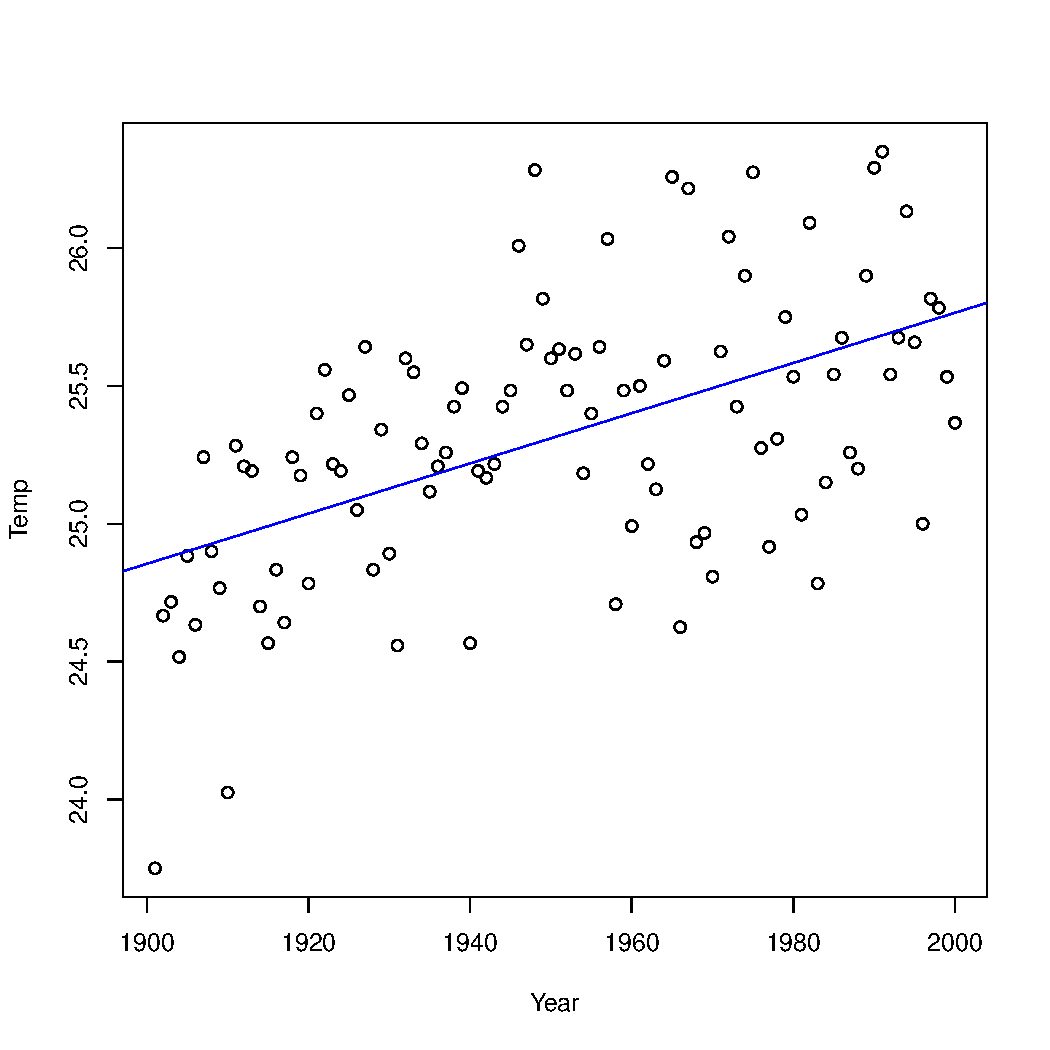
\includegraphics[width=.7\linewidth]{keywest.pdf}
        \centering
        \caption{This graph demonstrates the annual temperatures from Key West in Florida, USA for the 20th century}
        \label{fig:mesh1}
    \end{minipage}%
    \begin{minipage}{.5\textwidth}
        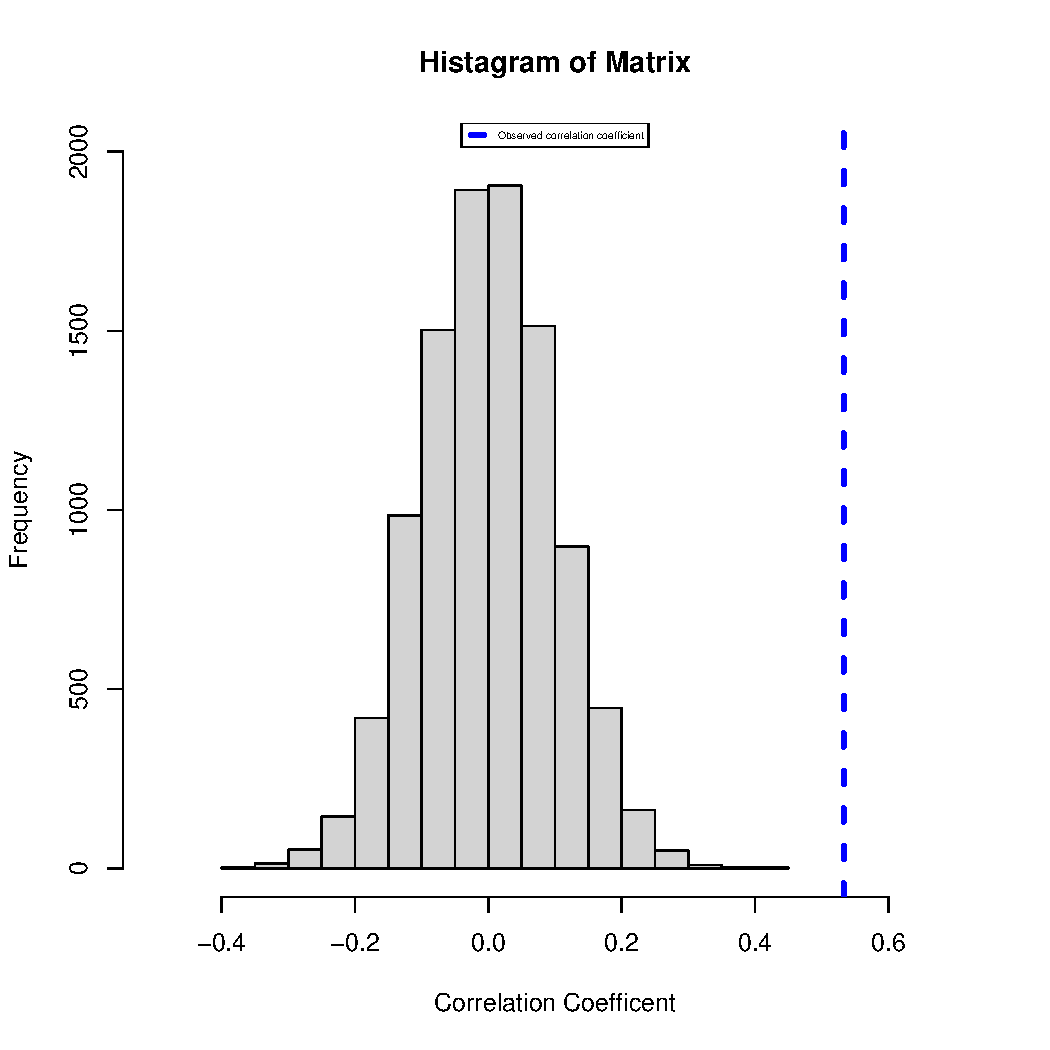
\includegraphics[scale=0.5]{histogram.pdf}
        \centering
        \caption{The distribution of random correlation coefficent calculated from reshuffling the temperatures}
        \label{fig:mesh2}
    \end{minipage}
    \end{figure}

\end{document}


